%!TEX root = ../../template.tex
%%%%%%%%%%%%%%%%%%%%%%%%%%%%%%%%%%%%%%%%%%%%%%%%%%%%%%%%%%%%%%%%%%%%
%% implementation_details.tex
%% Implementation Details section for Proposed Model and Implementation
%%%%%%%%%%%%%%%%%%%%%%%%%%%%%%%%%%%%%%%%%%%%%%%%%%%%%%%%%%%%%%%%%%%%

\section{Implementation Details}
\label{sec:ProposedModelImplementationDetails}

With the architecture defined in Section~\ref{sec:ProposedModelArchitecturalOverview}, this section focuses on how the platform was actually built. It goes over the technologies chosen, how the backend code is organized across services, and how everything is deployed using containers.

\subsection{Technology Stack}
Table~\ref{tab:technology-stack} summarizes the main technologies used across the platform.

\begin{table}[htbp]
    \centering
    \caption{Technology stack of the platform.}
    \label{tab:technology-stack}
    \begin{tabular}{l l l}
        \hline
        \textbf{Layer}         & \textbf{Technology} & \textbf{Role}                                  \\
        \hline
        \multicolumn{3}{l}{\textbf{\textit{Cloud Infrastructure}}}                                    \\[2pt]
        \gls{MQTT} broker      & EMQX                & Device telemetry ingestion                     \\
        Event backbone         & Apache Kafka        & Inter-service event backbone                   \\
        Database               & TimescaleDB         & Time-series and relational storage             \\
        Cache                  & Redis               & Distributed caching and real-time coordination \\
        Object storage         & MinIO               & S3-compatible object storage                   \\[4pt]
        \multicolumn{3}{l}{\textbf{\textit{Cloud Platform}}}                                          \\[2pt]
        Backend framework      & NestJS              & Microservice framework (TypeScript)            \\
        \gls{ORM}              & Prisma              & Database access and migrations                 \\[4pt]
        \multicolumn{3}{l}{\textbf{\textit{Edge Node}}}                                               \\[2pt]
        Edge framework         & NestJS              & Edge node application (Raspberry Pi)           \\
        Edge \gls{MQTT} broker & Mosquitto           & Local \gls{MQTT} broker                        \\
        Edge database          & SQLite              & Local persistence for offline resilience       \\[4pt]
        \multicolumn{3}{l}{\textbf{\textit{Frontend Application}}}                                    \\[2pt]
        Web framework          & Next.js             & Web application (React 19, TailwindCSS)        \\[4pt]
        \multicolumn{3}{l}{\textbf{\textit{Deployment}}}                                              \\[2pt]
        Containerization       & Docker              & Container orchestration (cloud and edge)       \\
        \hline
    \end{tabular}
\end{table}

The backend runs on NestJS, a TypeScript framework that supports building microservices with built-in Kafka consumers, \gls{HTTP} servers, and WebSocket gateways. Since TypeScript is also used within Next.js on the frontend, the same language covers the entire codebase. NestJS's module system made it possible for each service to follow the same patterns and share common code, which helped maintaining seven separate services. Its dependency injection also makes it clear what each service depends on.

The database layer uses TimescaleDB. Section~\ref{sec:ProposedModelDataModelAndStorageDesign} explains why relational and time-series storage were combined in a single PostgreSQL-based instance.

MinIO serves as the object store for binary files uploaded by devices. The Protocol Adapter stores files in MinIO and emits metadata events to Kafka, as described in Section~\ref{sec:ProposedModelDataFlowAndInteraction}. The bucket is created automatically on startup if it does not exist.

For inter-service communication, the platform relies on Apache Kafka as described in Section~\ref{sec:ProposedModelArchitecturalOverview}. Inside the monorepo, a shared \texttt{kafka} library keeps all topic names and consumer group identifiers in one place so they stay consistent across services.

\subsection{Backend Service Organization}
The backend is organized as a NestJS monorepo. The \texttt{apps/} directory contains seven services, each running as its own container: the \gls{API} gateway, the authentication service, the ingestion service, the analytics service, the notifications service, the read service, and the protocol adapter. Every service has its own entry point, modules, and configuration.

To avoid duplicating code across services, shared logic is placed in libraries under \texttt{libs/}. There are five of these. The \texttt{prisma} library holds the database schema and generated client, used by every service that talks to TimescaleDB. The \texttt{kafka} library keeps broker configuration, topic names, and consumer group identifiers in a single place. \texttt{contracts} defines the TypeScript interfaces for Kafka messages, so producers and consumers agree on the format at compile time. The remaining two, \texttt{common} and \texttt{dto}, contain utility functions and \gls{REST} \gls{API} response interfaces respectively.

This setup is a middle ground between having a separate repository per service and putting everything in one tightly coupled codebase. Each service can be built and deployed independently, but when something shared changes, like a database migration or a new event field, it can be updated in all the services at the same time. NestJS helps here because each service only imports the modules it actually needs, making the dependencies between them explicit.

The edge node lives in a separate repository. It is also a NestJS application, with Mosquitto instead of EMQX, SQLite instead of TimescaleDB, and no Kafka. Keeping it apart from the cloud monorepo avoids mixing edge-specific dependencies into the cloud build.

\subsection{Deployment and Orchestration}
Docker Compose manages the entire platform with twenty-one containers on a shared network, so they find each other by container name. Six of these are infrastructure dependencies: EMQX, Kafka, TimescaleDB, Redis, MinIO, and Mailhog (for development email testing). Nine are application containers: the seven backend microservices, the \gls{MQTT}-Kafka bridge, and a Kafka \gls{UI} for broker inspection. The remaining six handle monitoring: Prometheus, Grafana, cAdvisor, and exporters for Kafka, Redis, and PostgreSQL. The overall deployment topology is shown in Figure~\ref{fig:deployment-topology}.

\begin{figure}[htbp]
    \centering
    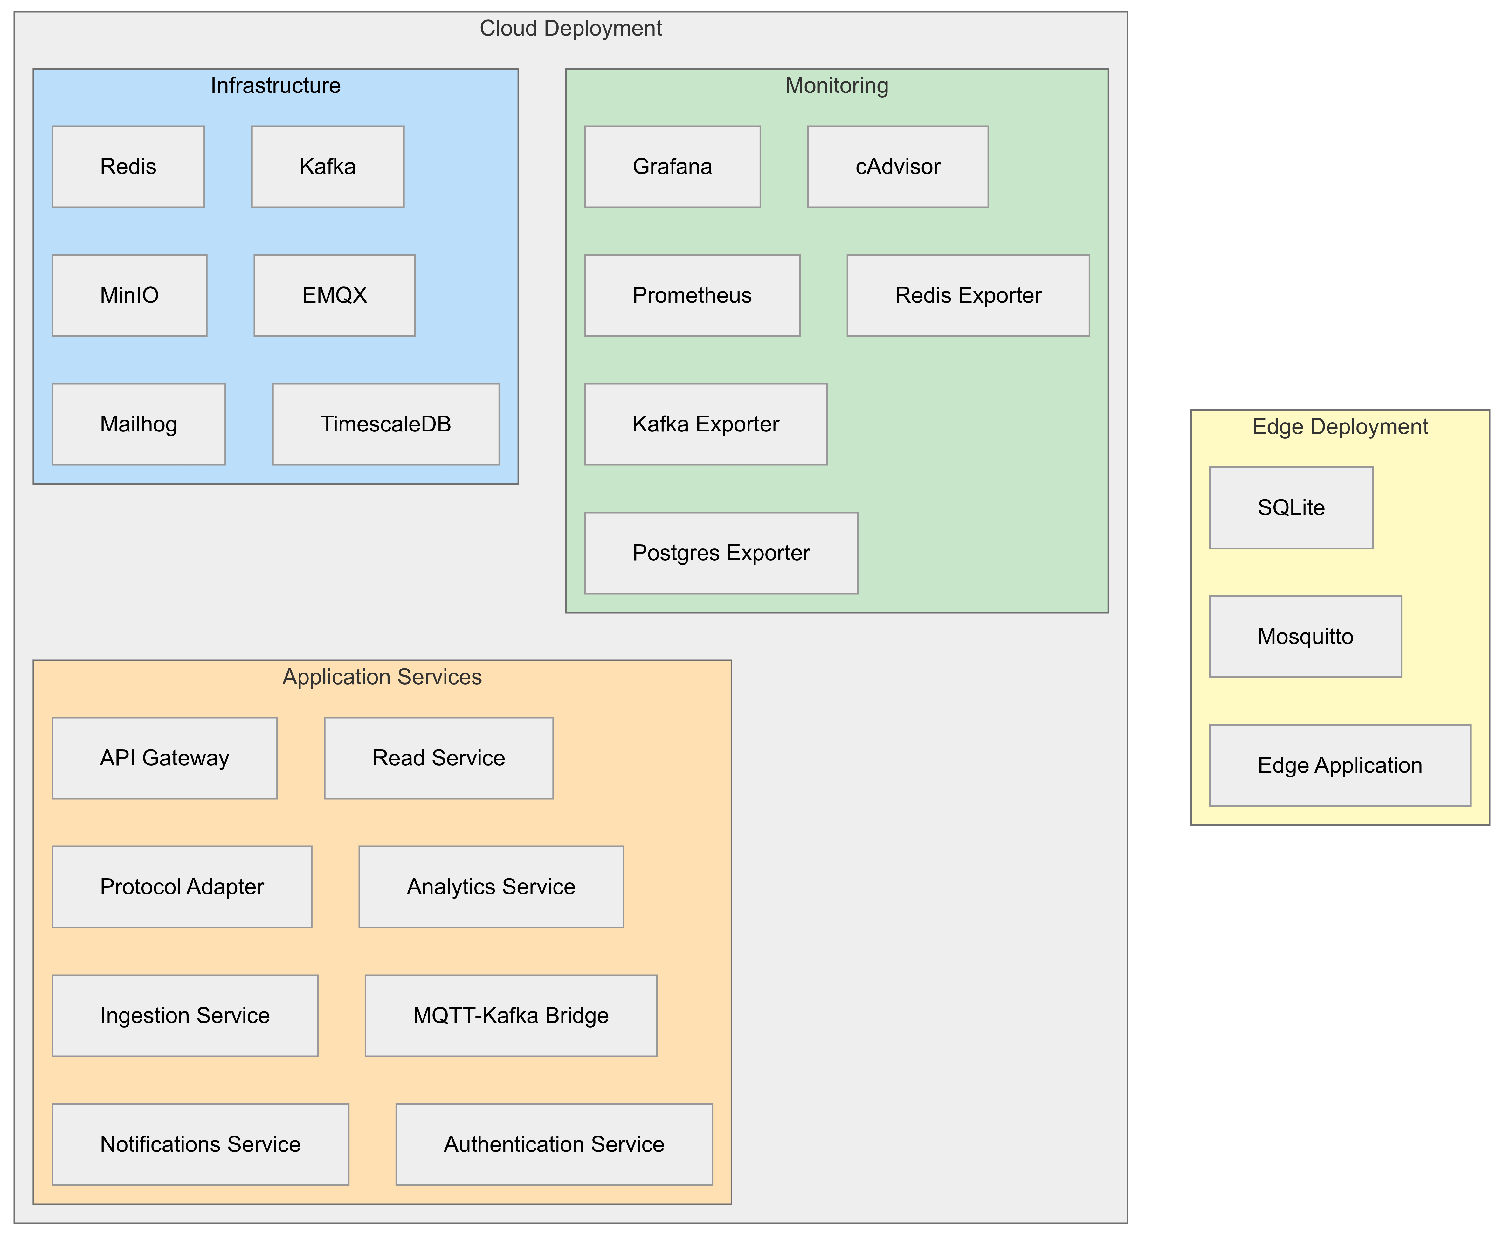
\includegraphics[width=\textwidth]{Chapters/Figures/Architectures/Deployment.pdf}
    \caption{Deployment topology of the platform, showing the cloud application services, infrastructure dependencies, monitoring stack, and separate edge deployment.}
    \label{fig:deployment-topology}
\end{figure}

Services need to start in the right order. TimescaleDB has to pass a health check before any service that needs the database can come up. Kafka must be healthy before any consumer or the \gls{MQTT}-Kafka bridge starts. Redis needs to be ready before the Read Service and Analytics Service, since both depend on it for caching. The \gls{API} gateway starts last because it proxies requests to all the other services. Docker Compose handles this through its dependency and health check configuration.

The edge node has its own, separate Docker Compose file with just two containers: the NestJS edge application and Mosquitto. To mimic constrained devices, the memory is limited to 1\,GB of \gls{RAM}, roughly 300\,MB for the application and 30\,MB for the broker, leaving room for the OS and SQLite. The \gls{RSA} public key for \gls{JWT} validation is mounted as a read-only volume, and the SQLite database sits on a host-mounted volume so data survives container restarts.

\subsection{Security Model: Asymmetric JWT Signing}
\label{subsec:jwt-rs256}
All \gls{JWT} signing and validation in the platform uses RS256 (\gls{RSA} with SHA-256), an asymmetric algorithm. The Authentication Service holds the private key and is the only component that can issue tokens. Every other component only receives the public key. This trust model is shown in Figure~\ref{fig:rs256-token-architecture}. Because the public key cannot create tokens, it can be safely distributed anywhere, including to the physically accessible edge node. A symmetric alternative like HS256 would require sharing a single secret with every validator, meaning any component that can verify a token could also forge one. Placing that secret on a remote, physically accessible device would be a serious security risk.

\begin{figure}[htbp]
    \centering
    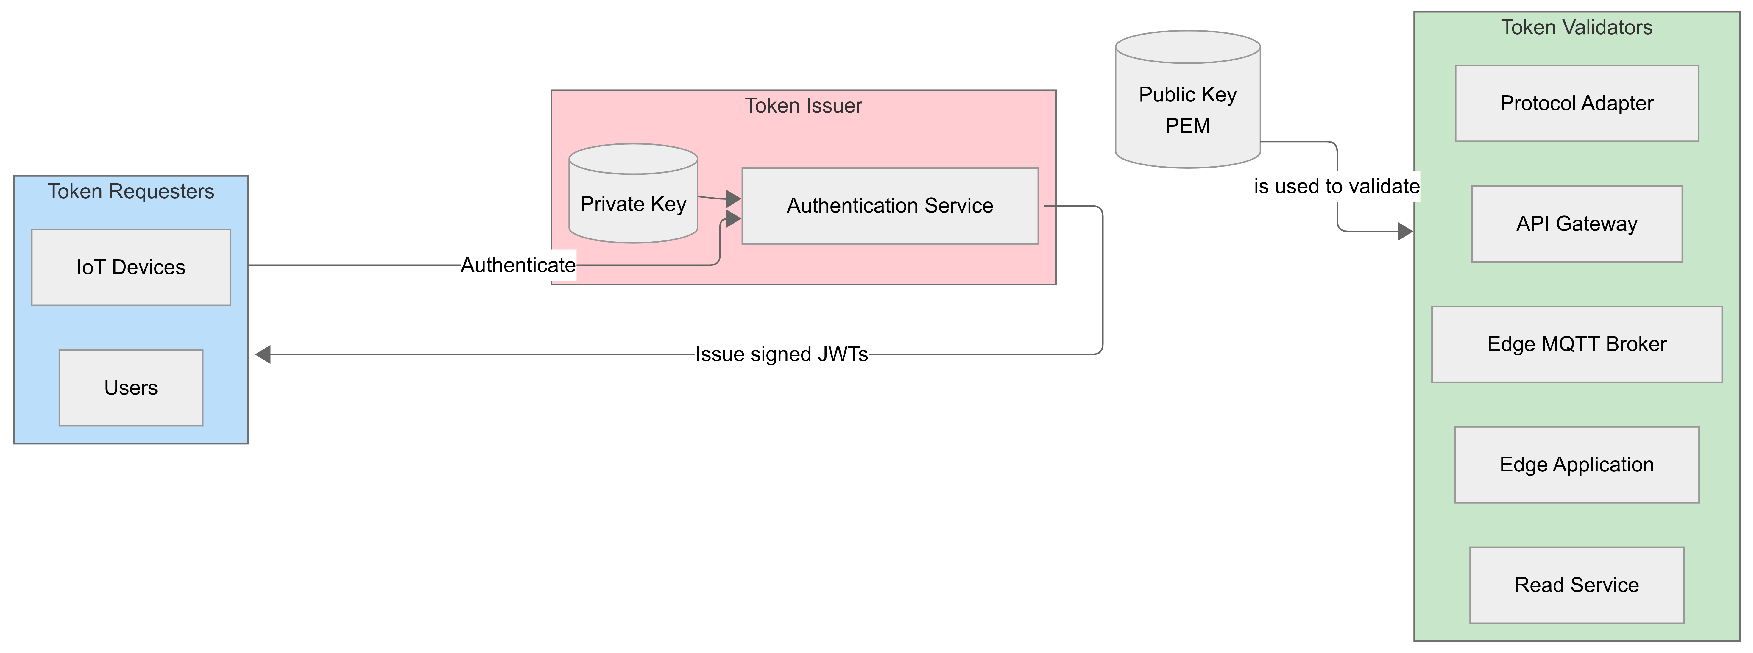
\includegraphics[width=\textwidth]{Chapters/Figures/Security/RS256TokenArchitecture.pdf}
    \caption{RS256 token issuance and validation architecture, showing that only the Authentication Service holds the private key while validating components use the public key for token verification.}
    \label{fig:rs256-token-architecture}
\end{figure}

With this setup, any component that receives the public key can verify tokens independently, without calling the Authentication Service. This includes the \gls{API} Gateway, the Protocol Adapter's \texttt{DeviceJwtGuard}, the Read Service for WebSocket handshake validation, the edge node's application, and the Mosquitto \texttt{mosquitto-go-auth} plugin for offline device authentication. The private key stays in the cloud, mounted as a secret in the Authentication Service container, and the public key is distributed as a \gls{PEM} file mounted read-only in each component that needs to check tokens.
